Questo capitolo è una sorta di manuale dell'utente: illustra come utilizzare ognuna delle funzionalità dell'applicazione. In Figura \ref{jama_home} è raffigurata la pagina principale di Jama, da cui si possono effettuare tutte le azioni disponibili in base all'utente loggato. La figura illustra la pagina principale per un Operatore; un Docente, per esempio, vedrebbe solo il tasto ''Visualizza i contratti''.
\begin{figure}[h]
	\centering
	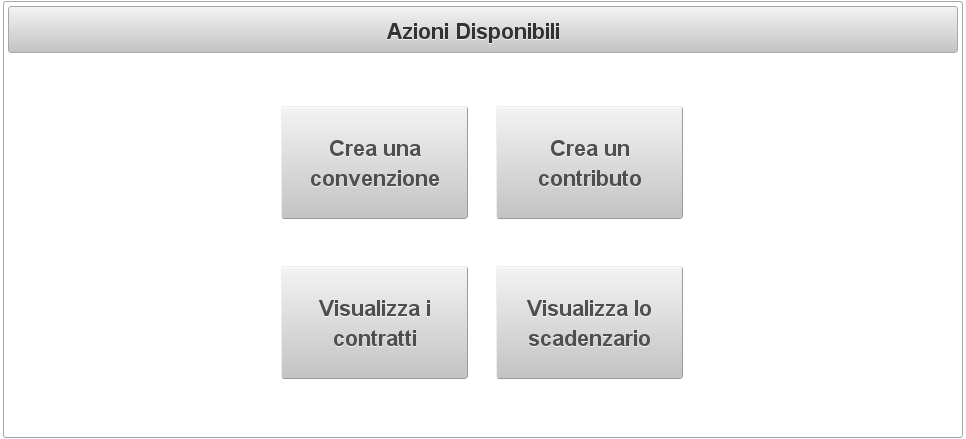
\includegraphics[width=13cm,height=6.5cm]{jama_home.png}
	\caption{La pagina principale di Jama}
	\label{jama_home}
\end{figure}

\section{Creare una convenzione}
\paragraph{}
Per creare una convenzione si clicca sul tasto ''Crea una convenzione''. Apparirà la finestra di Figura \ref{jama_create_agreement_tab_data}, in cui l'Operatore può inserire i dati principali della convenzione. Cliccando sul pulsante ''Next'', apparirà la finestra di Figura \ref{jama_create_agreement_tab_sharetable}, in cui l'utente può inserire i dati della Tabella di Ripartizione. Cliccando sul pulsante ''Annulla'', come si può intuire, l'inserimento della convenzione viene annullato e si ritorna alla pagina principale.\newline
Tornando alla Figura \ref{jama_create_agreement_tab_data}, accanto al menù ''Responsabile Scientifico'' è presente il pulsante ''Aggiungi'' che, se cliccato, farà apparire il pop-up di Figura \ref{jama_chief_scientist_popup}, che consente di inserire un nuovo Responsabile Scientifico all'interno dell'applicazione. Il campo ''Matricola'' del pop-up serve ad associare tale Responsabile Scientifico all'utente che effettivamente è legato ad esso; ad esempio, se la matricola del Professor Enrico Vicario è D593, inserendo il Responsabile Scientifico ''Enrico Vicario'' con matricola ''D593'' il Professor Vicario, effettuando il login con la sua matricola, potrà consultare le sue effettive convenzioni.\newline
Il pulsante ''Aggiungi'' accanto al menù delle Ditte è simile al precedente, con l'unica differenza che le Ditte non hanno matricola e non sono associate ad alcun utente.\newline

\begin{figure}[h]
	\centering
	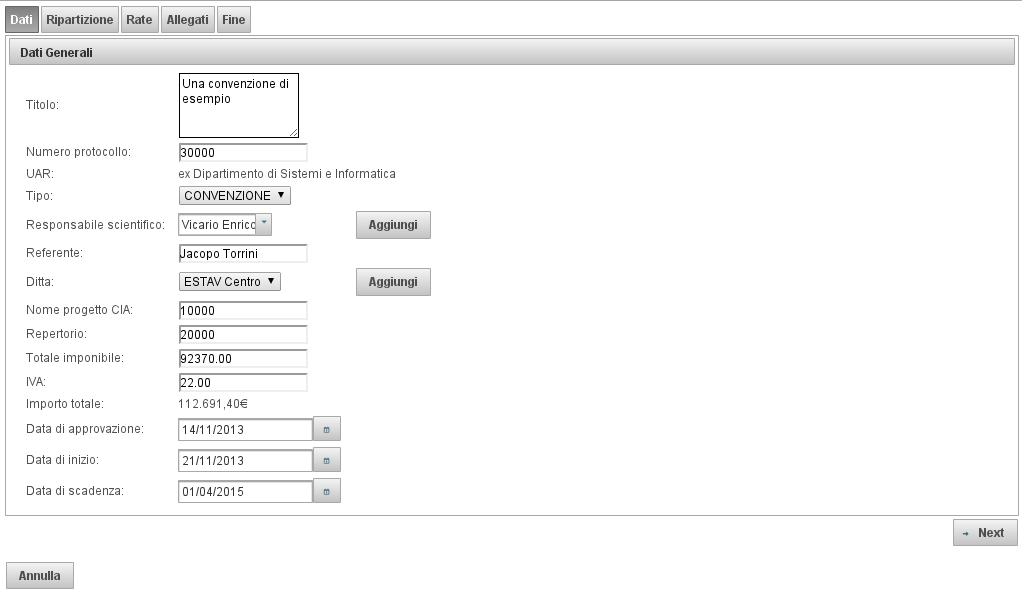
\includegraphics[width=13cm,height=6.5cm]{jama_create_agreement_tab_data.png}
	\caption{I dati principali di una convenzione}
	\label{jama_create_agreement_tab_data}
\end{figure}

\paragraph{}
Tornando alla Tabella di Ripartizione - Figura \ref{jama_create_agreement_tab_sharetable} - qualora la quota del ''Personale'' sia diversa da 0, si dovrà specificare almeno un Responsabile Scientifico nella tabella in fondo alla pagina. Per fare ciò, si seleziona il Responsabile Scientifico e la sua quota, e si clicca sul pulsante ''Aggiungi''. Com'è ovvio, sommando le quote della tabella si deve ottenere il 100\%, altrimenti verrà segnalato un errore e non si potrà continuare l'inserimento.\newline
Nel caso in cui si voglia cambiare un Responsabile Scientifico o la sua quota, si dovrà prima rimuovere la riga della tabella tramite il pulsante ''Rimuovi'', per poi inserire la nuova quota.\newline
Cliccando il pulsante ''Next'' si arriverà alla schermata della gestione delle rate, illustrata in Figura \ref{jama_installment_management}.
\paragraph{}
\begin{figure}
	\centering
	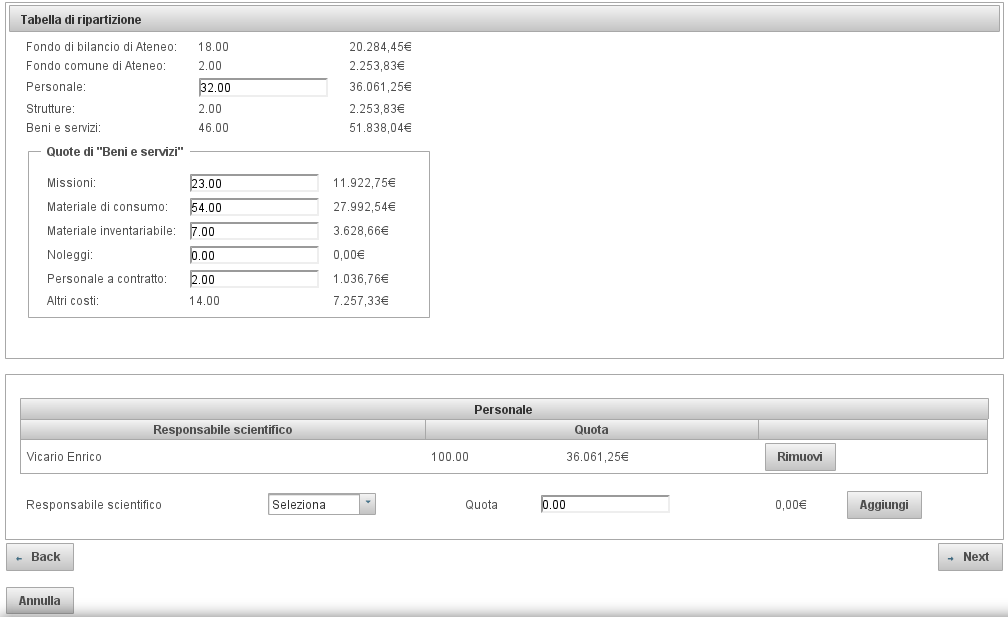
\includegraphics[width=13cm,height=6.5cm]{jama_create_agreement_tab_sharetable.png}
	\caption{La tabella di ripartizione}
	\label{jama_create_agreement_tab_sharetable}
\end{figure}

\begin{figure}
	\centering
	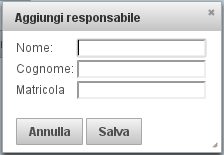
\includegraphics{jama_chief_scientist_popup.png}
	\caption{Il pop-up per inserire un nuovo Responsabile Scientifico nel database}
	\label{jama_chief_scientist_popup}
\end{figure}
La pagina di gestione delle rate è molto semplice: in alto vi è la lista delle rate della convenzione, che si inseriscono, prevedibilmente, con il pulsante ''Aggiungi una rata''. Parleremo in dettaglio di come si aggiunge una rata nei paragrafi successivi.\newline
Cliccando il pulsante ''Next'', si arriva alla pagina degli allegati, mostrata in Figura \ref{jama_attachments_management}.
\paragraph{}
La schermata di gestione degli allegati è fondamentalmente identica a quella delle rate: in alto è presente la lista a cui aggiungere gli allegati tramite il pulsante ''Aggiungi''.\newline
Gli allegati inseriti si possono cancellare e scaricare rispettivamente attraverso i due bottoni visibili in figura, che appaiono
andando col mouse sopra la riga in questione.
\paragraph{}
Infine, cliccando ancora una volta sul pulsante ''Next'' - sì, si fa presto a diventare ripetitivi a scrivere un manuale utente - si arriva alla schermata conclusiva, mostrata in Figura \ref{jama_agreement_save}. Cliccando sul pulsante ''Salva'', la convenzione viene finalmente registrata.

\begin{figure}
	\centering
	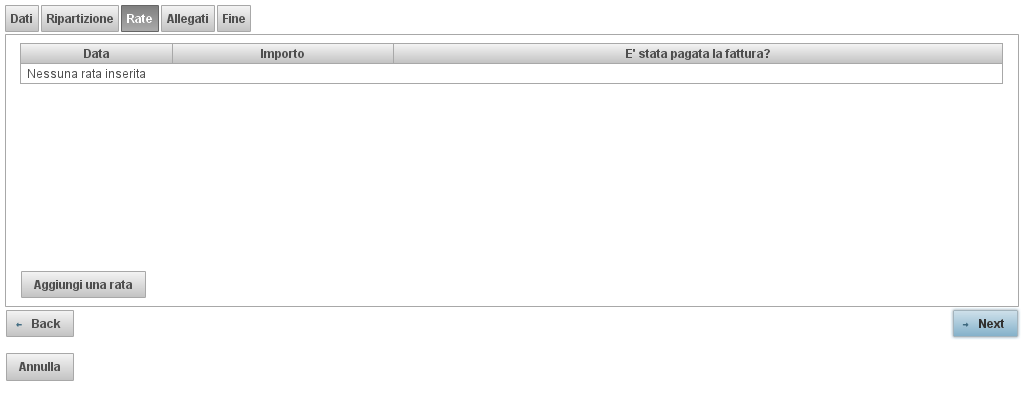
\includegraphics[width=13cm,height=6.5cm]{jama_installment_management.png}
	\caption{La pagina di gestione delle rate}
	\label{jama_installment_management}
\end{figure}

\begin{figure}
	\centering
	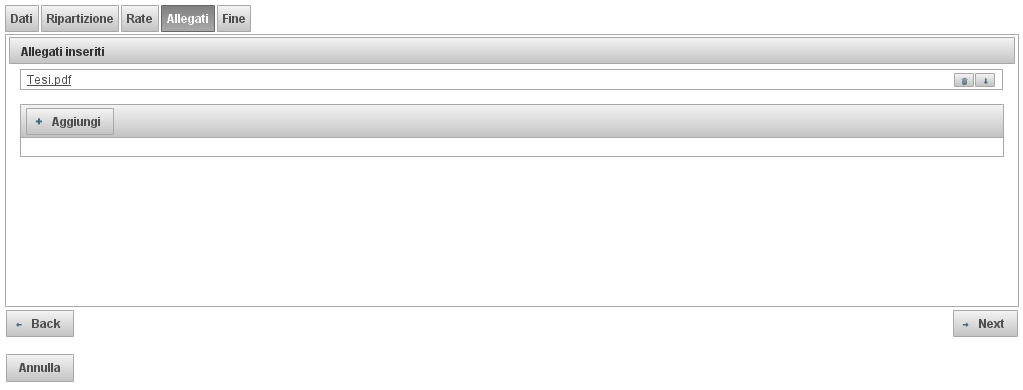
\includegraphics[width=13cm,height=6.5cm]{jama_attachments_management.png}
	\caption{La pagina di gestione degli allegati}
	\label{jama_attachments_management}
\end{figure}

\begin{figure}
	\centering
	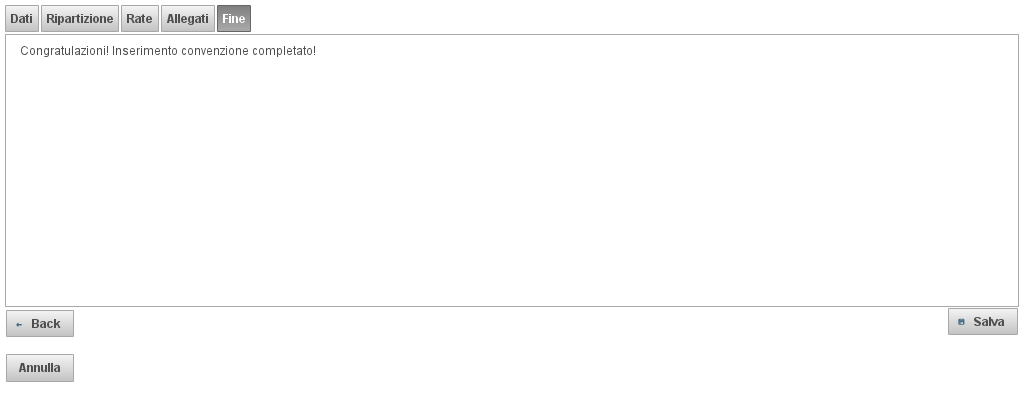
\includegraphics[width=13cm,height=6.5cm]{jama_agreement_save.png}
	\caption{La pagina conclusiva}
	\label{jama_agreement_save}
\end{figure}

